\documentclass[letter, 11pt, onecolumn]{article}


\usepackage{geometry}
\geometry{letterpaper, margin=1in}
\usepackage{amsmath}
\usepackage{amssymb}  
\usepackage{amsthm}
\usepackage{ulem} 
\usepackage{graphicx}
\usepackage{subfig} 
\usepackage{hyperref}

\graphicspath{ {images/} }


\title{\vspace{-2.0cm}PH 481 Physical Optics: Lab 1 }
\author{John L Waczak \\ Lab Partner: Darlene Focht}
\date{\today}


\begin{document}
	\maketitle
	
	\section*{Introduction}
		 This first lab explores the properties of thin lenses, introduces lab equipment and software, and provides practice for common optical equipment. Four separate experiments were performed. In the first, a 100 mm positive lens was examined in order to experimentally verify the focal length and magnification. The second experiment demonstrated a technique for aligning the optical axis in a u-shaped beam geometry. Finally, we used equipment to create a Keplerian telescope and then measured the pixel width of a camera using software techniques and the focused image of a ruler. 
	
	\section*{Theory} 
		\subsection*{1.1 Thin Lenses} 
		The two most common types of lenses used in the optics laboratories are the positive, double convex converging lens and the negative, double concave diverging lens. \\
			\begin{figure}[h!]
				\centering
				\subfloat{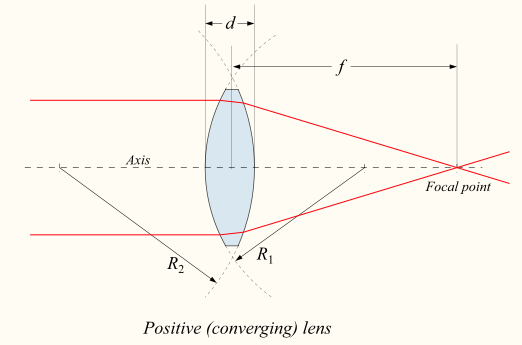
\includegraphics[width=0.45\columnwidth]{positive_lens}}
				\subfloat{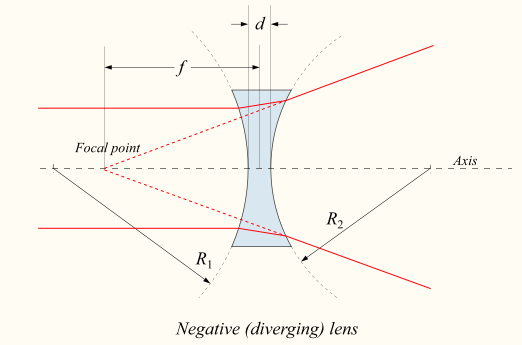
\includegraphics[width=0.45\columnwidth]{negative_lens}}
				\caption{Common lens types and their geometries [1]}
			\end{figure} 
		
		\noindent Figure 1 shows images of both the positive and negative lens. The defining characteristic for each of these objects is called the focal length. This number is determined by the geometry of each individual lens and can be used to predict where the lens will project an image (real or virtual) via the equation: 
			\begin{equation}
				\frac{1}{f} = \frac{1}{d_o}+\frac{1}{d_i}
			\end{equation}
		
		\noindent Depending on the object distance, the image can be magnified. This equation is is given by:
			\begin{equation}
				M = \frac{-d_i}{d_o}
			\end{equation}
			
		\subsection*{1.3 Expanding Laser Beams}
		A Keplerian telescope is a device used to magnify incoming light however for our purposes, we can use the geometry of a Keplerian telescope to serve as a beam expander. The system consists of two positive lenses called the objective and the eyepiece which work together as shown in the following figure.
			\begin{figure}[h!]
				\centering
				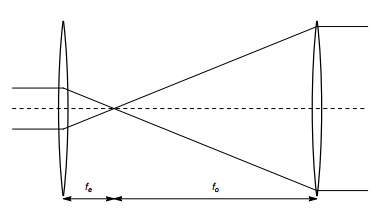
\includegraphics[width=0.45\columnwidth]{telescope}
				\caption{Keplerian telescope. Image taken from [2]}
			\end{figure}
		Coherent beam expansion occurs when the lenses are separated by the sum of their focal lengths. The magnification of the beam expander is given as:	
			\begin{equation}
				M = \frac{f_0}{f_e}
			\end{equation}
			
		\subsection*{1.4 Familiarization with Lab Equipment}
		A useful tool for studying optical phenomena are cameras. Many of our subsequent experiments will depend on this tool. The important metric governing the maximum resolution of the camera is the width of one pixel. 
	
	\section*{Experiment} 
		\subsection*{1.1 Thin Lenses} 
		The 100 mm positive lens was mounted on the optical rail at 50 cm. Starting 200 mm (20 cm) away from the lens a target slide containing a 10 x 10 grid of 1 mm squares was placed on one side of the lens. A desk lamp was used to send light through the target and lens to the opposite side of the rail where a white placard was used to determine where the image was sharp enough. The width of the image of the 25 mm band from the target was marked on the placard in order to help determine the magnification of the image. The length between the lens and image were then recorded. This process was then repeated for 10 mm (1cm) increments until the image could no longer be focused. From this data, the focal length can be verified by fitting image distance versus object distance as governed by equation 1. 
		
		\subsection*{1.2 Alignment Project}
		The second experiment served to provide experience at aligning the optical axis of a laser the u-shaped geometry pictured below: \\
		
			\begin{figure}[h!]
				\centering
				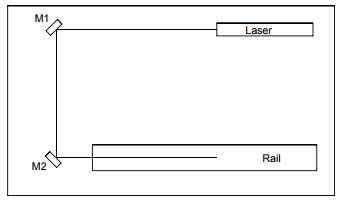
\includegraphics[width=0.4\columnwidth]{u_geometry}
				\caption{Alignment Geometry. Image taken from [2]}
			\end{figure}
		\noindent Two mirrors were employed, as seen in figure three, to bend the path of the laser light towards the optical rail. Each mirror contains two adjustments; one for each axis that enables the beam to be aligned. After ensuring the height of the laser was roughly 14.5 cm (a sufficient height for the lenses), both irises were closed and M1 was manipulated to align the laser with the center of the leftmost iris on the optical rail. Afterwards the left iris was opened and M2 was manipulated until the laser beam passed through both the left and right iris. Small adjustments were made until symmetric halo could be seen on each iris and the second could me moved back and forth without changing the level of the beam. 
		
		\subsection*{1.3 Expanding Laser beam} 
		As instructed by our TA, rather than using two positive lenses to make the Keplerian beam expander, we instead made use of a -25mm negative diverging lens for the eyepiece and a 75 mm positive lens for the objective. This slight change in geometry dramatically reduced the width of the entire system which we were instructed would be helpful in future experiments where we needed to use the expanded beam for some other purpose. \\ 
		
		\noindent Rather than place the lenses so that the distance between them was the sum of their focal lengths. The positive objective lens was placed 50 mm from the negative eyepiece so that the objective was one focal length away from the virtual image of the eyepiece. This enabled the same expansion as if two positive lenses were used as in figure 2. To determine if the beam was actually collimated, escaping light was reflected back through the system and towards the laser so that the objective could be moved until a focus was achieved. 
		
		\subsection*{1.4 Familiarization with Lab Equipment} 
		In order to determine the pixel size of the camera, the same 100 mm positive lens was placed on the optical rail. The target slide with the 1 mm squares was placed on a stand two focal lengths (200 mm) away from the lens. The camera was then moved to roughly the same distance on the opposite side of the lens. The exposure settings were manipulated to achieve good lighting and then the camera was moved until focus was found. \\ 
		
		Using the ImageJ program, a region of the image was selected so that the edges of one of the squares of the target were visible. Then using the plot profile tool, the number of pixels per 1 mm was determined. 
		
	\section*{Results}
		\subsection*{1.1 Thin Lenses}
		The following table shows the recorded image distances at various object distances as well as the measured magnification and expected magnification based off on equation [2]. \\
			\begin{figure}[h!]
				\centering
				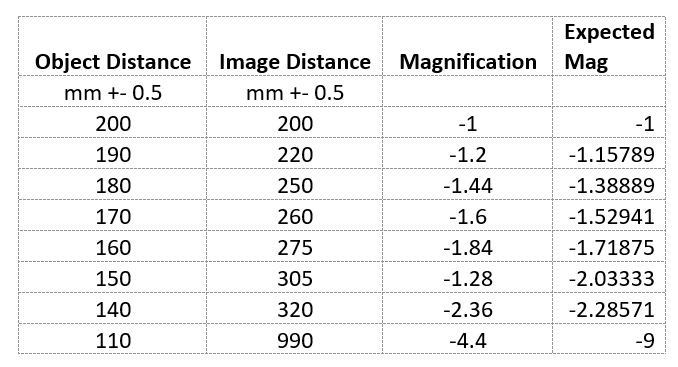
\includegraphics[width = 0.6\columnwidth]{table1}
				\caption{table of values}
			\end{figure} 
		
		\noindent Using Dr. McIntyre's $\chi^2$ excel sheet as a guide, the theoretical fit for the data was determined by varying the value of the focal length. The experimental data as well as the best fit line are shown in the following figure. 
			\begin{figure}[h!]
				\centering
				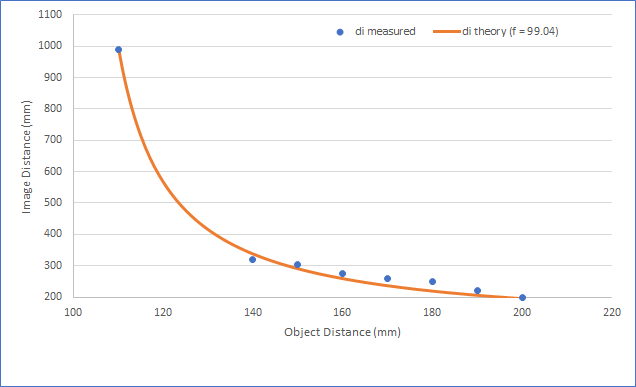
\includegraphics[width=0.75\columnwidth]{graph1}
				\caption{experimental and theoretical image distances}
			\end{figure}
		
		\subsection*{1.3 Expanding Laser Beams}
		Using the reflection of the resultant light back towards the laser beam, we we found that that the beam expander was focused when the objective lens was 55 mm away from the negative eyepiece. The width of the laser beam was measured directly before entering the eyepiece to be 4 mm initially. After exiting the apparatus, the beam had a width of 12.5 mm. Using formula [3] this gives a magnification of:
			\begin{equation}
				M_{\text{telescope}}=\frac{12.5}{4} = 3.125
			\end{equation}
		
		\subsection*{1.4 Familiarization with Lab Equipment}
		After focusing the the image in the lens, the target slide grid was captured with the USB camera. The following is the captured image that was used to deduce the pixel size: 
			\begin{figure}[h!]
				\centering
				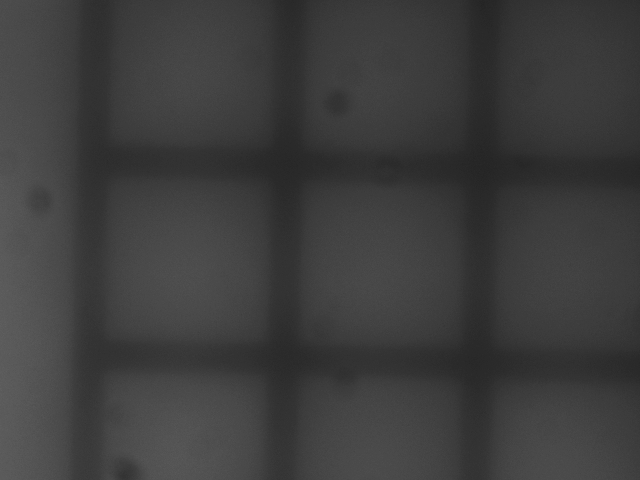
\includegraphics[width=0.5\columnwidth]{pixelSize}
				\caption{focused target grid}
			\end{figure}
			
		Using the plot profile command in ImageJ on the bitmap of figure 6, a grays scale plot was generated for a section of the image that reflects the dark bars on the image.  
			\begin{figure}[h!]
				\centering
				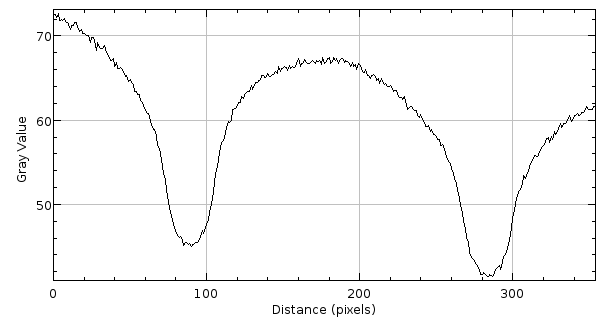
\includegraphics[width=0.75\columnwidth]{pixelSizePlot}
				\caption{gray scale plot showing grid with in pixels}
			\end{figure}
		
		Reading off the pixel distance for the two minima yields values of 89 and 285 for a total width of $285-89=196$. This means the pixel width is as follows: 
			\begin{equation}
				\frac{1\cdot10^{-3}\text{ mm}}{196 \text{ pixels}} = 5.1 \mu  \text{m/pixel}
			\end{equation}
			
		\noindent After completing this pixel measurement, Darlene and I ran out of time to complete the stage measurements and photo diode experiment.
	\section*{Discussion} 
	In our first experiment, we were able to fit our data to a lens of positive 99.04 focal length. For a 100 mm lens this is well within our experimental uncertainties. If we consider that the worst relative measurement uncertainty was $\frac{0.5\text{ mm}}{110\text{ mm}} \approx 0.01$ then using this as a weakest link metric for the experiment, our result was within 1 percent of the// actual value. \\
	
	\noindent The second experiment actually proved to be one of the most difficult as we nearly had the entire system aligned when we realized that the laser was positioned too low for the optical equipment. This meant that we had to recalibrate. One of most helpful tricks during this process were to ensure the path from the laser to M1 and then M2 fell parallel to a line of screw holes in the table as this was easy to visually confirm. Despite using the method of varying M1 to fit the first iris and then M2 to fit the second we still had some trouble ensuring the path of the beam was perfectly level along the optical axis.\\
	
	\noindent In the third experiment we had success using the negative diverging lens as the eyepiece. Manipulating the objective lens led to coherence at a slightly larger distance than was expected. The measured magnification was 3.125 which is quite close to the theoretical value of 3 obtained by dividing the objective focal length by the eyepiece focal length. We can likely attribute this difference to the propagation of the $\pm 0.5$ mm measurement uncertainty in our magnification calculation as well as the fact that this geometry meant the measured distance between the two lenses was very small (50 mm). \\
	
	\noindent In our final experiment we measured the pixel width to be on the scale of 5 microns which was confirmed to be on the right order by our lab TA. Sources of potential uncertainty in this measurement are the fact that the magnetic stand was used to hold the camera instead of putting it on the optical rail. This made measuring the lens-camera distance slightly more difficult. 
	
	\section*{Conclusions}
	We were able to successfully complete all experiments except for the final two due to time constraints. Experimental data was shown to compare to theoretical values within reasonable level of uncertainty. Each experiment enabled the exploration of optical equipment including lasers, lenses, mirrors, cameras, and others. 
	
	\section*{References} 
	[1] \url{https://en.wikipedia.org/wiki/Lens_(optics)} \\ 
	\noindent[2] \url{http://physics.oregonstate.edu/~mcintyre/COURSES/ph481/LABS/Lab1.pdf}
\end{document}











































